% :wrap=soft:maxLineLen=80:tabSize=2:indentSize=2:

\documentclass[a4paper,10pt]{article}

\usepackage[usenames,dvipsnames,x11names,rgb]{xcolor}
\usepackage{tikz}
\usetikzlibrary{mindmap}
\usepackage[english,UKenglish]{babel}
\usepackage{graphicx}
\usepackage{amsmath}
\usepackage{amsfonts}

\begin{document}

\begin{figure}[htp]
    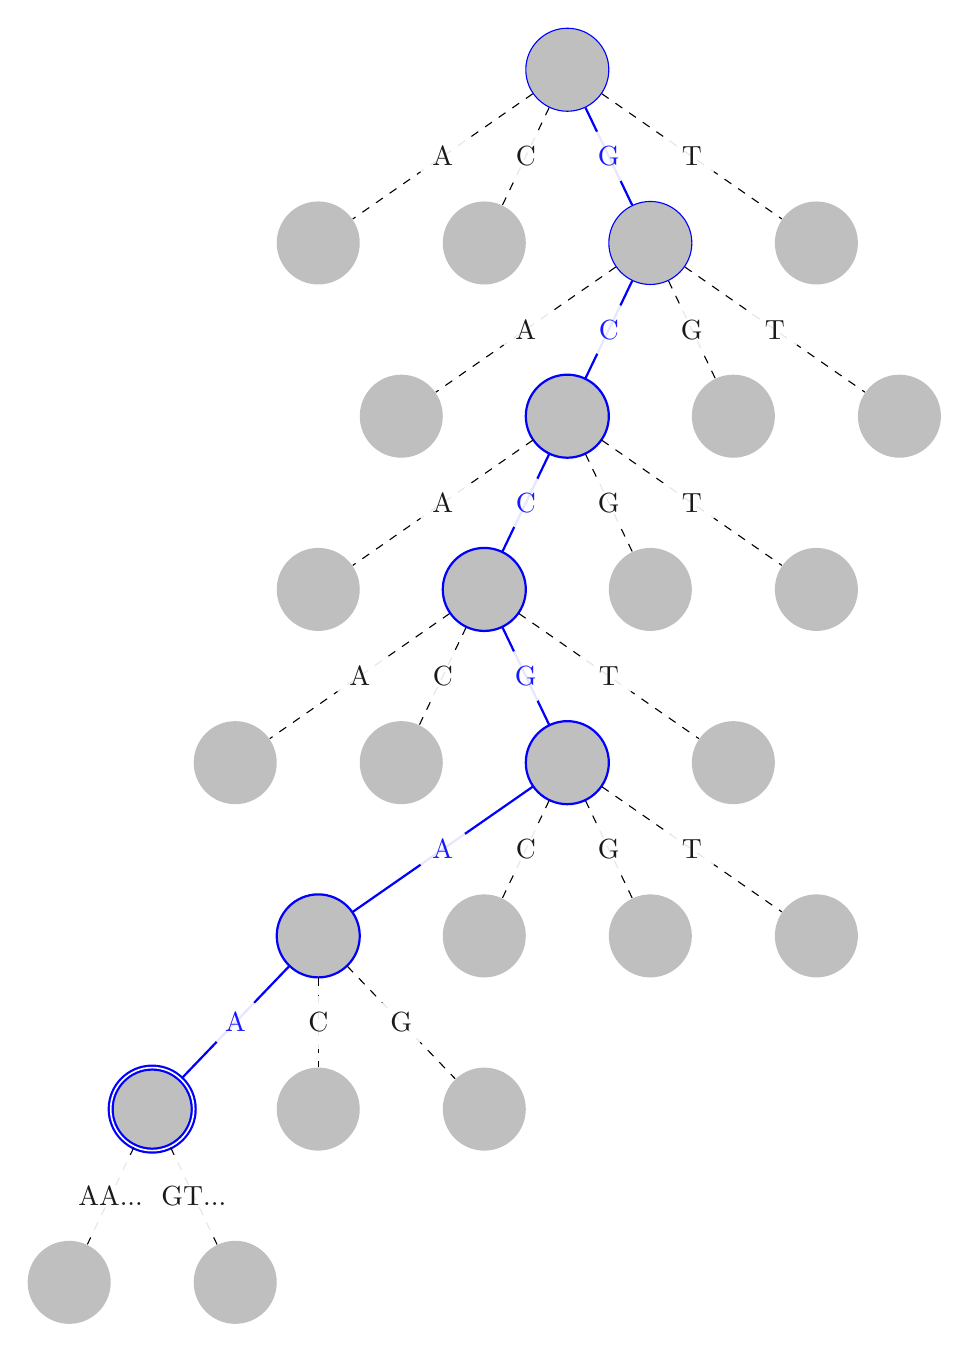
\begin{tikzpicture}[
        align=flush center,
        edge label/.style={fill=white,fill opacity=0.9,shape=circle},
        edge on path/.style={thick,blue,solid},
        edge off path/.style={thin,black,dashed},
        node/.style={fill=gray!50,shape=circle,minimum size=3em},
        node off path/.style={node},
        node on path/.style={node,draw=blue},
        last node on path/.style={node on path,double,thick},
        %grow cyclic,
        %level 1/.style={level distance=2.5cm,sibling angle=90},
        %level 2/.style={text width=2cm, font=\footnotesize, level distance=3cm,sibling angle=30},
        %level 3/.style={text width=2cm, font=\footnotesize, level distance=3cm,sibling angle=30},
        grow=down,
        level 1/.style={level distance=2.2cm,sibling distance=6em},
        %level 2/.style={level distance=3cm,sibling distance=3em},
        %level 3/.style={level distance=3cm,sibling distance=1em},
    ]
        \node[node on path] {}
  child {
  node[node off path] {}
  edge from parent[edge off path] node[edge label] {A}
  }
  child {
  node[node off path] {}
  edge from parent[edge off path] node[edge label] {C}
  }
  child {
  node[node on path] {}
    child {
    node[node off path] {}
    edge from parent[edge off path] node[edge label] {A}
    }
    child {
    node[node on path] {}
      child {
      node[node off path] {}
      edge from parent[edge off path] node[edge label] {A}
      }
      child {
      node[node on path] {}
        child {
        node[node off path] {}
        edge from parent[edge off path] node[edge label] {A}
        }
        child {
        node[node off path] {}
        edge from parent[edge off path] node[edge label] {C}
        }
        child {
        node[node on path] {}
          child {
          node[node on path] {}
            child {
            node[last node on path] {}
                                                                                                                                                                                                                                                                                                                                                                                                                                                                                                child {
                                                                                                                                                                                                                                                                                                                                                                                                                                                                                                node[node off path] {}
                                                                                                                                                                                                                                                                                                                                                                                                                                                                                                edge from parent[edge off path] node[edge label] {AA...}
                                                                                                                                                                                                                                                                                                                                                                                                                                                                                                }
                                                                                                                                                                                                                                                                                                                                                                                                                                                                                                                                                                                                                                                                                                                                                                                                                                                                                                                                                                                                                                                                                                                                                                                                                                                                                                                                                                                                                                                                                                                                                                                                                                                                                                                                                                                                                                                                                                                                                                                                                                                                                                                                                                                                                                                                                                                                                                                                                                                                                                                                                                                                                                                                                                                                                                                child {
                                                                                                                                                                                                                                                                                                                                                                                                                                                                                                                                                                                                                                                                                                                                                                                                                                                                                                                                                                                                                                                                                                                                                                                                                                                                                                                                                                                                                                                                                                                                                                                                                                                                                                                                                                                                                                                                                                                                                                                                                                                                                                                                                                                                                                                                                                                                                                                                                                                                                                                                                                                                                                                                                                                                                                                node[node off path] {}
                                                                                                                                                                                                                                                                                                                                                                                                                                                                                                                                                                                                                                                                                                                                                                                                                                                                                                                                                                                                                                                                                                                                                                                                                                                                                                                                                                                                                                                                                                                                                                                                                                                                                                                                                                                                                                                                                                                                                                                                                                                                                                                                                                                                                                                                                                                                                                                                                                                                                                                                                                                                                                                                                                                                                                                edge from parent[edge off path] node[edge label] {GT...}
                                                                                                                                                                                                                                                                                                                                                                                                                                                                                                                                                                                                                                                                                                                                                                                                                                                                                                                                                                                                                                                                                                                                                                                                                                                                                                                                                                                                                                                                                                                                                                                                                                                                                                                                                                                                                                                                                                                                                                                                                                                                                                                                                                                                                                                                                                                                                                                                                                                                                                                                                                                                                                                                                                                                                                                }
            edge from parent[edge on path] node[edge label] {A}
            }
            child {
            node[node off path] {}
            edge from parent[edge off path] node[edge label] {C}
            }
            child {
            node[node off path] {}
            edge from parent[edge off path] node[edge label] {G}
            }
          edge from parent[edge on path] node[edge label] {A}
          }
          child {
          node[node off path] {}
          edge from parent[edge off path] node[edge label] {C}
          }
          child {
          node[node off path] {}
          edge from parent[edge off path] node[edge label] {G}
          }
          child {
          node[node off path] {}
          edge from parent[edge off path] node[edge label] {T}
          }
        edge from parent[edge on path] node[edge label] {G}
        }
        child {
        node[node off path] {}
        edge from parent[edge off path] node[edge label] {T}
        }
      edge from parent[edge on path] node[edge label] {C}
      }
      child {
      node[node off path] {}
      edge from parent[edge off path] node[edge label] {G}
      }
      child {
      node[node off path] {}
      edge from parent[edge off path] node[edge label] {T}
      }
    edge from parent[edge on path] node[edge label] {C}
    }
    child {
    node[node off path] {}
    edge from parent[edge off path] node[edge label] {G}
    }
    child {
    node[node off path] {}
    edge from parent[edge off path] node[edge label] {T}
    }
  edge from parent[edge on path] node[edge label] {G}
  }
  child {
  node[node off path] {}
  edge from parent[edge off path] node[edge label] {T}
  }
;

    \end{tikzpicture}
    \caption{ \label{fig:myfigure}
      My figure.
    }
\end{figure}

\end{document}
